%This work is licensed under the Creative Commons
%Attribution-ShareAlike 4.0 International License. To view a copy of
%this license, visit http://creativecommons.org/licenses/by-sa/4.0/ or
%send a letter to Creative Commons, PO Box 1866, Mountain View, CA
%94042, USA.

%This work is licensed under the Creative Commons
%Attribution-ShareAlike 4.0 International License. To view a copy of
%this license, visit http://creativecommons.org/licenses/by-sa/4.0/ or
%send a letter to Creative Commons, PO Box 1866, Mountain View, CA
%94042, USA.

%\documentclass[gray,handout, pdftex, 11pt]{beamer}
%\documentclass[handout, pdftex, 11pt]{beamer}

\documentclass[pdftex, 11pt]{beamer}

\usepackage[utf8]{inputenc}
\usepackage[T1]{fontenc}
\usepackage{lmodern}
%\usepackage[italian]{babel}
\usepackage{graphicx}
\usepackage{listings}
\usepackage{microtype}
\usepackage{acronym}
\usepackage{array}
\usepackage{tikz}
\usetikzlibrary{shapes, chains, scopes, shadows, positioning, arrows,
  decorations.pathmorphing, calc}

\colorlet{c1}{green!20}
\colorlet{c2}{blue!10}
\colorlet{drawColor}{black!50}
\colorlet{commentColor}{green!70!black!90}

\tikzstyle{oval}=[ellipse, align=center, drop shadow, draw=drawColor, fill=white]
\tikzstyle{rect}=[rectangle, rounded corners=2pt, align=center, drop
shadow, draw=drawColor, fill=white]
\tikzstyle{comment}=[text=commentColor,font=\itshape]
\tikzstyle{textLab}=[]
\tikzstyle{arrow}=[->, very thick, >=stealth', draw=black!80]
\tikzstyle{darrow}=[->, dash pattern=on 3pt off2pt, very thick, >=stealth', draw=black!80]
\tikzstyle{fStartEnd}=[ellipse, align=center, drop shadow, draw=drawColor, fill=white]
\tikzstyle{fInput}=[trapezium, trapezium left angle=70, trapezium right angle=110,
align=center, drop shadow, draw=drawColor, fill=white]
\tikzstyle{fProcess}=[rectangle, align=center, drop shadow, draw=drawColor, fill=white]
\tikzstyle{fSelection}=[diamond, shape aspect=3, align=center, drop
shadow, draw=drawColor, fill=white]
\tikzstyle{fOutput}=[tape, tape bend top=none, align=center, drop shadow, draw=drawColor, fill=white]
\tikzstyle{mem}=[rectangle, align=center, draw=drawColor, fill=white]
\tikzstyle{clo}=[cloud, aspect=2, align=center, drop shadow, draw=drawColor, fill=white]

\lstdefinestyle{customc}{
   language=C,
   % basicstyle=\small\ttfamily\bfseries,
   basicstyle=\ttfamily,
   keywordstyle=\color{blue}\ttfamily,
   stringstyle=\color{red}\ttfamily,
   commentstyle=\color{green}\ttfamily,
   morecomment=[l][\color{magenta}]{\#},
   % breaklines=false,
    breaklines=true, breakatwhitespace=false,
   frameround=fttt,
   frame=trBL,
   backgroundcolor=\color{yellow!20},
   numbers=left,
   stepnumber=1,    
   firstnumber=1,
   numberfirstline=true,
   numberstyle=\tiny\color{black!50},
   xleftmargin=2em,
   framexleftmargin=1.5em
   % linewidth=8cm,
}

\lstnewenvironment{cblock}[1][]
{
  \lstset{
    style=customc,
    #1
  }
}{}

\newcommand{\cfile}[2][]{
  \lstinputlisting[style=customc, #1]{#2}
}

\definecolor{links}{HTML}{2A1B81}
\hypersetup{colorlinks,linkcolor=links,urlcolor=links}

\definecolor{links}{HTML}{2A1B81}
\hypersetup{colorlinks,linkcolor=,urlcolor=links}


\mode<presentation>{
  %-------------------------1
  \usetheme{Boadilla}
  \usecolortheme{beaver}
  %-------------------------1
  %-------------------------2
  %\usetheme{Goettingen}
  %\usecolortheme{sidebartab}
  %-------------------------2
  %\useoutertheme[right]{sidebar}
  %\usefonttheme{default}
  \setbeamercovered{transparent}
  %\setbeameroption{show notes on second screen=right}
  \setbeamertemplate{navigation symbols}{}
  \setbeamertemplate{footline}{}

  \bibliographystyle{abbrv}  
  %\renewcommand\bibfont{\scriptsize}
  \setbeamertemplate{bibliography item}{\textbullet}
  \setbeamertemplate{itemize item}{\checkmark}
  \setbeamertemplate{itemize subitem}{-}
  \setbeamertemplate{enumerate items}[default]
  \setbeamertemplate{sections/subsections in toc}[square]
}

\subtitle{Logical Computational Thinking}
\institute[Tecnológico de Monterrey]{
  
\includegraphics[width=5cm]{img/logoTEC.jpg}\\[5mm]
  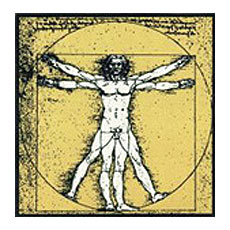
\includegraphics[width=1cm]{img/logoLEO.jpg}
  Scuola Leonardo Da Vinci (Firenze)
}

\author[Stefano Martina]{
  %\\[0.2cm]
  \textbf{Stefano MARTINA}\\
  {\small stefano.martina@gmail.com}
}

\titlegraphic{\tiny
  \href{http://creativecommons.org/licenses/by-sa/4.0/}{
\includegraphics[width=1cm]{img/logoCC.png}}
  This work is licensed under a
  \href{http://creativecommons.org/licenses/by-sa/4.0/}{Creative
    Commons Attribution-ShareAlike 4.0 International License}.}


\title[Lesson 2]{\textbf{Lesson 2 - Introduction to C language}}
\date[10/9/15]{\flushright 10 September 2015}

\begin{document}

\begin{frame}[plain]
  \titlepage
\end{frame}

\begin{frame}
  \frametitle{Review}
  \begin{center}
    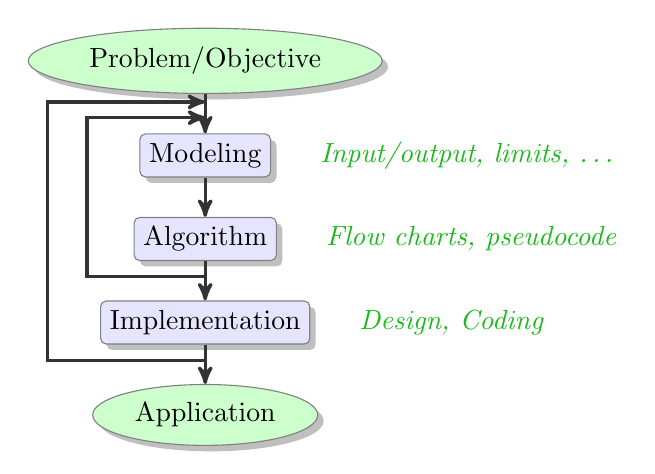
\begin{tikzpicture}[node distance=5mm]
      \node (realProb) [oval, fill=c1] {Problem/Objective};
      \node (model) [rect, fill=c2, below=of realProb] {Modeling};
      \node [comment, right=of model] {Input/output, limits, \dots};
      \draw [arrow] (realProb) -- (model);
      \node (algorithm) [rect, fill=c2, below=of model] {Algorithm};
      \node [comment, right=of algorithm] {Flow charts, pseudocode};
      \draw [arrow] (model) -- (algorithm);
      \node (implementation) [rect, fill=c2, below=of algorithm] {Implementation};
      \node [comment, right=of implementation] {Design, Coding};
      \draw [arrow] (algorithm) -- (implementation);
      \node (application) [oval, fill=c1, below=of implementation] {Application};
      \draw [arrow] (implementation) -- (application);
      \draw [arrow] ($ (implementation.south) + (0,-2mm) $) -- ++(-20mm,0) |- ($ (model.north) + (0,4mm) $);
      \draw [arrow] ($ (algorithm.south) + (0,-2mm) $) -- ++(-15mm,0) |- ($ (model.north) + (0,2mm) $);
    \end{tikzpicture}
  \end{center}
\end{frame}

\begin{frame}
  \frametitle{Model}
  \begin{center}
    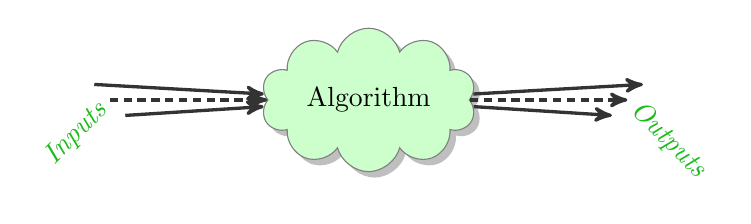
\begin{tikzpicture}[node distance=20mm]
      \node (inputs) [comment, rotate=45] {Inputs};
      \node (algorithm) [clo, fill=c1, right=of inputs] {Algorithm};
      \node (outputs) [comment, right=of algorithm, rotate=315] {Outputs};
      \draw [arrow] (inputs.north east) -- (algorithm);
      \draw [darrow] (inputs.east) -- (algorithm);
      \draw [arrow] (inputs.south east) -- (algorithm);
      \draw [arrow] (algorithm) -- (outputs.north west);
      \draw [darrow] (algorithm) -- (outputs.west);
      \draw [arrow] (algorithm) -- (outputs.south west);
    \end{tikzpicture}    
  \end{center}
\end{frame}

\begin{frame}
  \frametitle{Algorithm}
  \begin{center}
        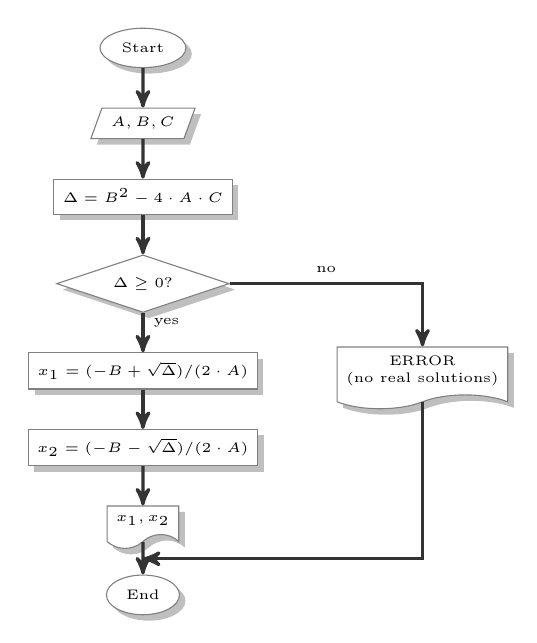
\begin{tikzpicture}[node distance=5mm, font=\tiny, auto]
      \node(start) [fStartEnd] {Start};
      \node(input) [fInput, below=of start] {$A,B,C$};
      \draw [arrow] (start) -- (input);
      \node(opD) [fProcess, below=of input] {$\Delta = B^2-4\cdot
        A\cdot C$};
      \draw [arrow] (input) -- (opD);
      \node(selection) [fSelection, below=of opD] {$\Delta\ge 0$?};
      \draw [arrow] (opD) -- (selection);
      \node(opX1T) [fProcess, below=of selection]
      {$x_1=(-B+\sqrt{\Delta})/(2\cdot A)$};
      \draw [arrow] (selection) -- node [near start] {yes} (opX1T);
      \node(opX2T) [fProcess, below=of opX1T]
      {$x_2=(-B-\sqrt{\Delta})/(2\cdot A)$};
      \draw [arrow] (opX1T) -- (opX2T);
      \node(outputErr) [fOutput, right=10mm of opX1T] {ERROR\\(no real
      solutions)};
      \draw [arrow] (selection) -| node [near start] {no} (outputErr);
      \node(output) [fOutput, below=of opX2T] {$x_1, x_2$};
      \draw [arrow] (opX2T) -- (output);
      \node(end) [fStartEnd, below=of output] {End};
      \draw [arrow] (output) -- (end);
      \draw [arrow] (outputErr) |- ($ (end.north) + (0,2mm) $);
    \end{tikzpicture}
  \end{center}
\end{frame}

\begin{frame}
  \frametitle{C language}
  \begin{figure}[h!]
    \centering
    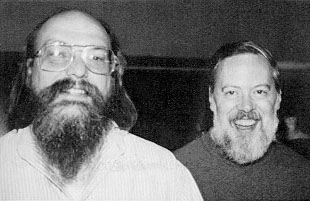
\includegraphics[width=5cm]{ken_n_dennis.jpg}
    \caption{Ken Thompson and Dennis Ritchie}
  \end{figure}
  \begin{block}{History}
    \begin{itemize}
    \item The language \alert{C} is developed in the 70's by Dennis Ritchie
    \item Along with the \alert{Unix} system, created by Ken Thompson and
      Dennis Ritchie in the same years
    \end{itemize}
  \end{block}
\end{frame}

\begin{frame}[fragile]
  \frametitle{Basics}
  \begin{block}{Blocks}
    \begin{cblock}
{
  ...
}
    \end{cblock}
    \begin{itemize}
    \item Good practice to \alert{indent} the code to the right every
      time a block is open, and to the left when is closed.
    \end{itemize}
  \end{block}
  \begin{block}{Comments}
    \begin{cblock}
//Single line comment

/* Multiple
lines
comments */
    \end{cblock}
  \end{block}
\end{frame}

\begin{frame}[fragile]
  \frametitle{Main and libraries}
  \begin{block}{Libraries}
    \begin{cblock}
#include<stdio.h>
#include<math.h>      
    \end{cblock}
    \begin{itemize}
    \item For including code defined elsewhere.
    \item Can be custom libraries or standard libraries like:
      \begin{itemize}
      \item \cc{stdio.h} stands for \emph{STandard Input Output} and
        provide basic interface with the terminal;
      \item \cc{math.h} provide some useful mathematical functions,
        like \cc{pow} and \cc{sqrt}.
      \end{itemize}
    \item The \cc{#include} directives must be write on top of the
      source file (before the main)
    \end{itemize}
  \end{block}
\end{frame}

\begin{frame}[fragile]
  \begin{block}{Main}
    \begin{itemize}
    \item Is the entry point for the program.
    \end{itemize}
    \begin{cblock}
int main(void) {
  ...
  return 0;
}
    \end{cblock}
    or
    \begin{cblock}
int main(int argc, char *argv[]) {
  ...
  return 0;
}
    \end{cblock}
  \end{block}
\end{frame}

\begin{frame}[fragile]
  \frametitle{Example}
  \cfile{hello_world.c}
\end{frame}

\begin{frame}[fragile]
  \frametitle{Variables}
  \begin{block}{Initialization}
    \begin{cblock}
int var1;            //default initial value
float var2 = 3.1415; //custom initial value
int var3, var4, var5;//multiple initialization
    \end{cblock}
  \end{block}
  \begin{itemize}
  \item C is \alert{case sensitive}, \cc{int} $\neq$ \cc{Int} $\neq$ \cc{INT}.
  \item Allowed names can contains \cc{[A-Z,a-z,0-9,_]}, cannot begin
    with a number.
  \item Good practices are: to use \alert{camel case} or \cc{_} for composed
    words, and to start with
    \alert{lower case}. I.e. \cc{camelCaseExample}.
  \item Also when possible define variables on method begin.
  \end{itemize}
\end{frame}

\begin{frame}[fragile]
  \frametitle{Variables}
    \begin{block}{Assignation}
    \begin{cblock}
var1 = 42;
    \end{cblock}
    \begin{itemize}
    \item Is possible to use also \alert{expressions} on the right of
      =
    \item Also with other variables or the same variable.
      \begin{cblock}
var3 = var4 + var5;
var3 = var3 - 1;
      \end{cblock}
    \end{itemize}
  \end{block}
\end{frame}

\begin{frame}
  \frametitle{Variable types}
  \begin{block}{Integer}
    \begin{tabular}{|l|l|r|r|}
      \hline
      \textbf{type} & \textbf{size} & \textbf{min value} & \textbf{max value} \\
      \hline
      \hline
      \cc{char} & 1 byte & -128 & 127 \\
      \hline
      \cc{short} & 2 bytes & -32,768 & 32,767 \\
      \hline
      \cc{int} & 4 bytes & -2,147,483,648 & 2,147,483,647 \\
      \hline
      \cc{long} & 8 bytes & \tiny -9,223,372,036,854,775,808 & \tiny 9,223,372,036,854,775,807\\
      \hline
      \hline
      \cc{unsigned char} & 1 byte & 0 & 255 \\
      \hline
      \cc{unsigned short} & 2 bytes & 0 & 65,535 \\
      \hline
      \cc{unsigned int} & 4 bytes & 0 & 4,294,967,295 \\
      \hline
      \cc{unsigned long} & 8 bytes & 0 & \tiny 18,446,744,073,709,551,615 \\
      \hline
    \end{tabular}
  \end{block}
  \begin{itemize}
  \item \cc{char} is used also for the characters of the \alert{ascii} table.
  \end{itemize}
\end{frame}

\begin{frame}
  \frametitle{Variable types}
  \begin{block}{Floating point}
    \begin{tabular}{|l|l|l|l|l|}
      \hline
      \textbf{type} & \textbf{size} & \textbf{min value} & \textbf{max value} & \textbf{epsilon} \\
      \hline
      \hline
      \cc{float} & 4 bytes & \tiny $1.175494\me^{-38}$ & \tiny $3.402823\me^{38}$
      & \tiny $1.192093\me^{-07}$ \\
      \hline
      \cc{double} & 8 bytes & \tiny $2.225074\me^{-308}$ & \tiny $1.797693\me^{308}$ & \tiny $2.220446\me^{-16}$ \\
      \hline
      \cc{long double} & 16 bytes & \tiny $3.362103\me^{-4932}$ & \tiny $1.189731\me^{4932}$ & \tiny $1.084202\me^{-19}$ \\
      \hline
    \end{tabular}
  \end{block}
  \begin{block}{Boolean}
    \begin{itemize}
    \item Is possible to use the type \cc{bool}, and the values
      \cc{true} and \cc{false}.
    \item You need to add \cc{\#include<stdbool.h>}.
    \item Not really useful because you can use any integer type with
      the values:
      \begin{itemize}
      \item $0$ for false;
      \item $\neq 0$ for true.
      \end{itemize}
    \end{itemize}
  \end{block}
\end{frame}

\begin{frame}[fragile]
  \frametitle{Operators (in priority order)}
  \begin{block}{Arithmetic}
    \begin{enumerate}
    \item \cc{*}, \cc{/}, \cc{\%};
    \item \cc{+}, \cc{-};
    \end{enumerate}
  \end{block}
  \begin{block}{Logic}
    \begin{enumerate}
      \setcounter{enumi}{1}
    \item \cc{!};
    \item \cc{<}, \cc{>}, \cc{<=}, \cc{>=}
    \item \cc{==}, \cc{!=};
    \item \cc{&&};
    \item \cc{||};
    \end{enumerate}
  \end{block}
  \begin{itemize}
  \item Is possible to change order with \cc{(} and \cc{)}, i.e.:
    \begin{cblock}
(a+b)*c
    \end{cblock}
  \end{itemize}
\end{frame}

\begin{frame}[fragile]
  \frametitle{Selections}
  \begin{center}
    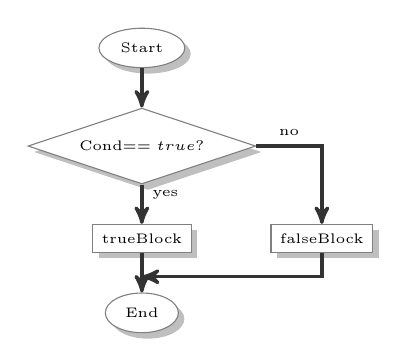
\begin{tikzpicture}[node distance=5mm, font=\tiny, auto]
      \node(start) [fStartEnd] {Start};
      \node(selection) [fSelection, below=of start] {\cc{Cond}$ == true$?};
      \draw [arrow] (start) -- (selection);
      \node(trueBlock) [fProcess, below=of selection] {\cc{trueBlock}};
      \draw [arrow] (selection) -- node [near start] {yes} (trueBlock);
      \node(falseBlock) [fProcess, right=10mm of trueBlock] {\cc{falseBlock}};
      \draw [arrow] (selection) -| node [near start] {no} (falseBlock);
      \node(end) [fStartEnd, below=of trueBlock] {End};
      \draw [arrow] (trueBlock) -- (end);
      \draw [arrow] (falseBlock) |- ($ (end.north) + (0,2mm) $);
    \end{tikzpicture}
  \end{center}  
  \begin{cblock}
if(cond) {
  trueBlock;
} else {
  falseBlock;
}
  \end{cblock}
\end{frame}

\begin{frame}[fragile]
  \frametitle{Selections}
  The \cc{else} block is optional.
  \begin{center}
    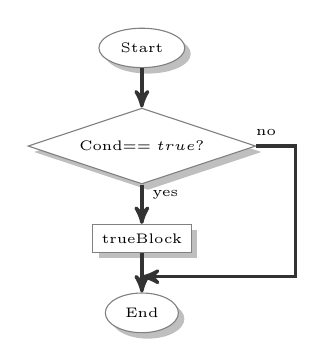
\begin{tikzpicture}[node distance=5mm, font=\tiny, auto]
      \node(start) [fStartEnd] {Start};
      \node(selection) [fSelection, below=of start] {\cc{Cond}$ == true$?};
      \draw [arrow] (start) -- (selection);
      \node(trueBlock) [fProcess, below=of selection] {\cc{trueBlock}};
      \draw [arrow] (selection) -- node [near start] {yes} (trueBlock);
      \node(end) [fStartEnd, below=of trueBlock] {End};
      \draw [arrow] (trueBlock) -- (end);
      \draw [arrow] (selection)
      -- node [near start] {no} ($ (selection.east) + (5mm,0) $)
      |- ($ (end.north) + (0,2mm) $);
    \end{tikzpicture}
  \end{center}  
  \begin{cblock}
if(cond) {
  trueBlock;
}
  \end{cblock}
\end{frame}

\begin{frame}[fragile]
  \frametitle{While iteration}
  \begin{center}
    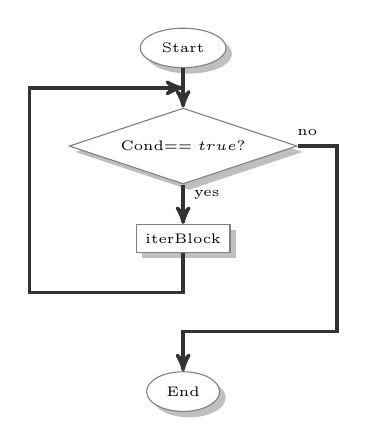
\begin{tikzpicture}[node distance=5mm, font=\tiny, auto]
      \node(start) [fStartEnd] {Start};
      \node(selection) [fSelection, below=of start] {\cc{Cond}$ == true$?};
      \draw [arrow] (start) -- (selection);
      \node(iterBlock) [fProcess, below=of selection] {\cc{iterBlock}};
      \draw [arrow] (selection) -- node [near start] {yes} (iterBlock);
      \node(end) [fStartEnd, below=15mm of iterBlock] {End};
      \draw [arrow] (iterBlock)
      -- ($ (iterBlock.south) - (0,5mm) $)
      -| ($ (selection.west) - (5mm,0) $)
      |- ($ (selection.north) + (0,2.5mm) $);
      \draw [arrow] (selection)
      -- node [near start] {no} ($ (selection.east) + (5mm,0) $)
      |- ($ (end.north) + (0,5mm) $)
      -- (end);
    \end{tikzpicture}
  \end{center}  
  \begin{cblock}
while(cond) {
  iterBlock;
}
  \end{cblock}  
\end{frame}

\begin{frame}[fragile]
  \frametitle{Do-while iteration}
  \begin{center}
    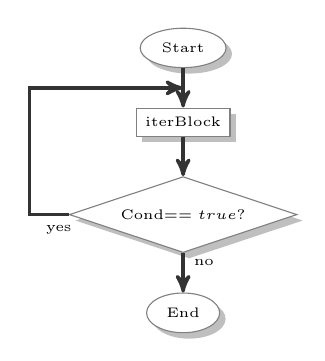
\begin{tikzpicture}[node distance=5mm, font=\tiny, auto]
      \node(start) [fStartEnd] {Start};
      \node(iterBlock) [fProcess, below=of start] {\cc{iterBlock}};
      \draw [arrow] (start) -- (iterBlock);
      \node(selection) [fSelection, below=of iterBlock] {\cc{Cond}$ == true$?};
      \draw [arrow] (iterBlock) -- (selection);
      \draw [arrow] (selection) 
      -- node [near start] {yes} ($ (selection.west) - (5mm,0) $)
      |- ($ (iterBlock.north) + (0,2.5mm) $);
      \node(end) [fStartEnd, below=of selection] {End};
      \draw [arrow] (selection) -- node [near start] {no} (end);
    \end{tikzpicture}
  \end{center}  
  \begin{cblock}
do {
  iterBlock;
} while(cond);
  \end{cblock}
\end{frame}

\begin{frame}[fragile]
  \frametitle{For iteration}
  \begin{cblock}
for(iniz; cond; oper) {
  iterBlock;
}
  \end{cblock}
  is equivalent to:
  \begin{cblock}
iniz;
while(cond) {
  iterBlock;
  oper;
}
  \end{cblock}
\end{frame}

\begin{frame}[fragile]
  \frametitle{For iteration example}
  \cfile{forTest.c}
\end{frame}

\begin{frame}
  \frametitle{User input/output}
  \begin{block}{Output: \cc{printf}}
    \cc{printf(format, var1, var2, ...);}
    \begin{itemize}
    \item \cc{format} is a string that contain the text to be send to output
    \item the format string can contains special chars using \cc{\\}
      \begin{itemize}
        \item \cc{\\\\}, \cc{\\"}, \cc{\\\%}, \cc{\\n} (for new line)
      \end{itemize}
    \item the format string can contains special \alert{format
        specifiers}
      \begin{itemize}
      \item for each specifier is necessary a corresponding variable
        \cc{var}
      \item the output string will be integrated with the value of the
        variables
      \end{itemize}
    \end{itemize}
  \end{block}
  \begin{block}{Input: \cc{scanf}}
    \cc{scanf(format, \&var);}
    \begin{itemize}
    \item \cc{format} is a string with only one \alert{format specifier}
    \item \cc{var} is a variable name (remember to add the special
      char \cc{\&})
    \item the input will be saved inside \cc{var}
    \end{itemize}
  \end{block}
\end{frame}

\begin{frame}
  \begin{block}{format specifiers}
    \begin{itemize}
    \item for each \alert{data type} corresponds a \alert{format specifier}
    \item a format specifier is \cc{\%[length][specifier]}
    \end{itemize}
    \begin{center}
      \small
      \begin{tabular}{|l||c|c|c|}
        \hline
        \multirow{2}{*}{\textbf{Length}} & \multicolumn{3}{c|}{\textbf{Specifier}} \\
        \cline{2-4}
        & \cc{d} & \cc{u} & \cc{f} (\cc{e} for $m\, 10^n$) \\
        \hline
        \hline
        (none) & \cc{int} & \cc{unsigned int} & \cc{float} \\
        \hline
        \cc{hh} & \cc{char} & \cc{unsigned char} & \\
        \hline
        \cc{h} & \cc{short} & \cc{unsigned short} & \\
        \hline
        \cc{l} & \cc{long} & \cc{unsigned long} & \cc{double} \\
        \hline
        \cc{L} & & & \cc{long double} \\
        \hline
      \end{tabular}
    \end{center}
  \end{block}
  For example:
  \begin{itemize}
  \item \cc{\%d} for \cc{int}
  \item \cc{\%hu} for \cc{unsigned short}
  \item \cc{\%Le} for \cc{long double} (expressed in scientific
    notation)
  \end{itemize}
\end{frame}

\begin{frame}[fragile]
  \cfile{printfScanfExample.c}
\end{frame}

\begin{frame}[fragile]
  \begin{bblock}
$ gcc printfScanfExample.c -o example
$ ./example 
Input\output
demonstration

Insert a rational number: 12.34
Insert a long integer: 123456
Rational is: 12.340000; integer is: 123456
Rational in scientific notation: 1.234000e+01
$
  \end{bblock}
\end{frame}
\end{document}